\documentclass[12pt]{article}
\usepackage[margin=1in]{geometry}
\usepackage{fancyvrb}
\usepackage{multicol}
\usepackage{hyperref}
\usepackage{amsmath}
\usepackage{amsfonts}

\usepackage[listings]{tcolorbox}

\definecolor{codegreen}{rgb}{0,0.6,0}
\definecolor{codegray}{rgb}{0.5,0.5,0.5}
\definecolor{codepurple}{rgb}{0.58,0,0.82}
\definecolor{backcolour}{rgb}{0.95,0.95,0.92}

\lstdefinestyle{mystyle}{
    language=Python,
    backgroundcolor=\color{backcolour},   
    commentstyle=\color{codegreen},
    keywordstyle=\color{magenta},
    numberstyle=\tiny\color{codegray},
    stringstyle=\color{codepurple},
    basicstyle=\ttfamily\footnotesize,
    breakatwhitespace=false,         
    breaklines=true,                 
    captionpos=b,                    
    keepspaces=true,                 
    numbers=left,                    
    numbersep=5pt,                  
    showspaces=false,                
    showstringspaces=false,
    showtabs=false,                  
    tabsize=2,
    escapechar=|,
    frame=single
}

\lstset{style=mystyle}

\newcommand{\showfig}[2]{
\noindent\includegraphics[width=\textwidth]{#1}
\centerline{#1}
}

\begin{document}
\sloppy
\centerline{\Large CSCI 111, Lab 9}
\centerline{\large Mandelbrot Explorer}

\showfig{mandX-1.393Y-0.408R0.5.png}


\begin{description}
\item[Due date:] Midnight, Tuesday, November 15, on Canvas.
No late work accepted.  

\item[File names:]  Names of files, functions, and variables, 
when specified,
must be EXACTLY as specified.  This includes simple mistakes such
as capitalization.

\item[Individual work:]  All work must be your own.  Do not share
code with anyone other than the instructor and teaching assistants.
This includes looking over shoulders at screens with the code open.
You may discuss ideas, algorithms, approaches, {\em etc.} with
other students but NEVER actual code.

\item[The Mandelbrot Set:]  The {\bf Mandelbrot set}
is the set of complex numbers $c$ such that the function
$f_c(z) = z^2 + c$ does not diverge to infinity
when iterated from $z=0$.  In other words, the
sequence $f_c(0), f_c(f_c(0)), f_c(f_c(f_c(0))), ...$
remains bounded in absolute value.

You can read a lot about this set online,
for example in Wikipedia:
\url{https://en.wikipedia.org/wiki/Mandelbrot_set},
and see many pretty pictures people have 
made by exploring this set and colorizing
it.

\item[Creating an image in pygame:]
I have provided a program, \lstinline{pygamecolors.py},
in the lab folder.
In that program I create the image of a simple gradient.
You will eventually use this framework to display 
the Mandelbrot set. 

Because Mandelbrot pictures can take a long
time to generate, this program  
illustrates how to make a complicated
image appear instantly, but roughly, and then gradually
refine it.  Notice that we start with very large pixels,
and reduce them by 1/2 each time we repeat.  Eventually
the image is as sharp as it can be, but with large sizes 
it takes quite a bit of time.

The program pauses between each pixelsize, just to give
you a chance to see the result before moving on.
This pause is entirely unnecessary and can be removed
in your versions.

Note that in this program I translated from screen coordinates
to `'normalized'' coordinates to make it easier to calculate
the colors.  Instead of $(x,y)$ going from $(0,0)$ to
$(width,height)$, as they do on the screen, they
go from $(0,0)$ to $(1,1)$.  This makes the color
computation much easier.  You will also transition
from screen coordinates to other coordinates in your
programs.

Finally, you should note that the program prints out
how long each render took, the times for each pixelsize,
and the total time for all pixelsizes together.
In one of my runs I got 4.4 seconds for the $1\times 1$
pixels, the final render, and 6.6 seconds for 
all renders together, from $128\times 128$ to 
$64\times 64$ to ... to $1\times 1$.
Thus, all 8 renders only took 2.2 seconds longer
than the one final one, or $2.2/6.6$ or about
33\% longer.  This seems a modest price to pay
for getting instant feedback about how the image
is going to appear.  You will notice that I've
enabled the user to quit the program before it
is finished.  If you see an image starting to
appear that is not at all what you expected,
you don't have to wait until the final, slow
image is complete to find out and quit!

\item[Mathematical aside (optional):]
The fact that 8
 renders only takes a bit longer
than one render is due to the following interesting
theorem (if you're not good at sums you can skip
this part):

\begin{align*}
\sum_{i=0}^n a^i = \sum_{i=1}^{n} a^i + a^0 &= \sum_{i=1}^{n} a^i + 1\\
\sum_{i=1}^{n}a^i &= \sum_{i=0}^{n} a^i - 1\\
a \sum_{i=0}^{n} a^i = \sum_{i=1}^{n+1} a^i &= a^{n+1} + \sum_{i=1}^{n} a^i  \\
               &= a^{n+1} + \sum_{i=0}^n a^i - 1   \\
(a-1)     \sum_{i=0}^n a^i  &= a^{n+1} -1\\
 \sum_{i=0}^n a^i  &= \frac{a^{n+1} -1}{a-1}       
\end{align*}      

Let's check this out.  If $a=2$ then
\begin{align*}
 2^0 + 2^1 + 2^3 + 2^4    &= 1 + 2 + 4+ 8\\
 &= 15= \frac{2^4-1}{2-1}
\end{align*} 
How about that.  

This is one of my favorite theorems, and really
important intuition in computer science.
When $a$ is very large,  $a - 1 \approx a$
and $a^{n+1} - 1 \approx a^{n+1}$, so, approximately,
\begin{align*}
\sum_{i=0}^{n} a^i &\approx a^n
\end{align*} 

This is extraordinary.  For large $a$, then
\[
a^0 + a^1 + a^2 + a^3 + a^4 + a^5 + a^6 + a^7 + a^8 + a^9 + a^{10} \approx a^{10}
\]
It's as if the smaller exponents don't even count!

Let's see what this has to do with our image viewer.
Each time we make the pixels half the width
and height of the previous pixels.  This means 
4 pixels fit into each previous pixel.  That
means we're computing 4 times as many pixels
each time around the pixelsize loop.  So, whatever
time the first loop took, the next one will take
four times longer.  And the next one four times longer than
that.  And so on.  So there's a factor of $4^i$
for the $i$th trip through the loop.  With $a=4$
\begin{align*}
\sum_{i=0}^{n} 4^i = \frac{4^{n+1} - 1}{4-1} 
 \approx \frac{4(4^n)}{3}\
 \approx 1.33(4^n)
\end{align*}
So, before I even wrote the program I expected
running all the pixelsize renders would only take
about 33\% longer than running just the final one.

The data proved me right.

You will see more amazing facts like this in your
study of algorithms.

\item[The Dot:] OK, now we know why that image rendering
program \lstinline{pygamecolors.py}
behaves like it does, and we know how to
get an image on the screen.  You should notice that
if you press the S key at any time the program
saves your image to a file, which is convenient.

Before we get to the Mandelbrot
set, let's handle a few of the mechanics so we
know what we're doing with a simple picture,
the spot.  

Our world consists, not of the Mandelbrot set,
but of a
spot of radius one, centered on the origin.
We will build a vewer to look at this marvelous
set, coloring the set blue and everything else 
green.  We will build a series of programs
that will allow us to examine this blue dot
in great detail.  

\centerline{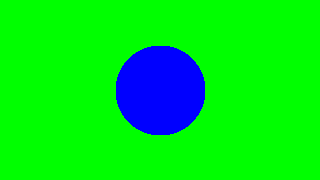
\includegraphics[scale=0.5]{spot}}

\item[Screen coordinates and world coordinates:]
The first challenge in producing the spot
is the transition between screen coordinates
and world coordinates.  The screen coordinates,
\lstinline{(i, j)} range from 0 to \lstinline{width}
and 0 to \lstinline{height}.

But we want to look at a circle that is centered
on the origin, with unit radius, and we want this
circle centered in our image as in the Figure.
Clearly, \lstinline{(0,0)} means different things
on the screen and in the world of our blue spot.

Also, a distance of 1, like the radius of the circle,
is clearly a distance of many pixels on our screen.
So a distance of 1 in world coordinates is not a distance
of one in screen coordinates.

The problem is we are using {\bf two coordinate systems}!
We have screen coordinates, and world coordinates.
Generally we will use \lstinline{(i, j)} to denote
screen coordinates in the range 
\lstinline{[0,width) x [0,height)},
and $(x,y)$ to denote real world coordinates
in the range $\mathbb{R} \times \mathbb{R}$,
the Cartesian plane of pairs of real numbers.

We need to transform screen coordinates into world
coordinates.  You will write the function
\begin{lstlisting}
def screenToWorld(i, j, width, height):
    ....
    return (x, y)
\end{lstlisting}
that will take screen coordinates of a point
and return world coordinates.  We may want
to include other parameters in this function, too,
later on.

At a minimum, screen coordinates 
\lstinline{(width/2, height/2)} should translate
to world coordinates $(0,0)$.  Can you see why?
If not, you may need to reread the last few paragraphs
a few times until you do.  If that doesn't work,
come and see me.

The height of our screen should show the blue dot,
and also some space above and below it.  Let's say,
since the blue dot has a radius of 1, there's space
of 1 unit above and below the dot.  That means
the screen is 4 units high in world coordinates.
If our screen is $640 \times 480$ in size, then
how many screen pixels correspond to 1 
unit distance in world coordinates?  

If you didn't get 120, then, again, stop
and reread, or talk to me, until you understand.

What about width?  The screen has an {\bf aspect ratio},
which is just \lstinline{width/height}.  Clearly,
if the height is \lstinline{x} units high in world
space, the width should
be \lstinline{x * aspectRatio} units wide, in world space.

So, if our screen is $640\times 480$, and 4 units
high in world space how wide is it
in world space?  If you didn't get $5\frac{1}{3}$, you
know what to do.

This should be enough information to
write your \lstinline{screenToWorld} function:
\begin{itemize}
\item Screen center is at world coordinates $(0,0)$
\item Screen height is 4 world units.
\item Screen width is \lstinline{aspect_ratio * 4}
in world units.
\end{itemize}
Write your \lstinline{screenToWorld} function and
test it out on some examples you've worked by hand,
like the ones above.
Keep working on the function and your examples
until you understand what this function is supposed
to do and how to do it.

\item[Test data:]  I ran \lstinline{screenToWorld}
with a screen centered at $(0,0)$ with 4 units
from top to bottom of screen, and a width and height
of (640, 480), and got these numbers for the input 
values of i and j:
\begin{lstlisting}
(0,0) => (-2.6666666666666665, 2.0)
(0,50) => (-2.6666666666666665, 1.5833333333333333)
(0,100) => (-2.6666666666666665, 1.1666666666666665)
(0,150) => (-2.6666666666666665, 0.75)
(50,0) => (-2.25, 2.0)
(50,50) => (-2.25, 1.5833333333333333)
(50,100) => (-2.25, 1.1666666666666665)
(50,150) => (-2.25, 0.75)
(100,0) => (-1.8333333333333333, 2.0)
(100,50) => (-1.8333333333333333, 1.5833333333333333)
(100,100) => (-1.8333333333333333, 1.1666666666666665)
(100,150) => (-1.8333333333333333, 0.75)
(150,0) => (-1.4166666666666665, 2.0)
(150,50) => (-1.4166666666666665, 1.5833333333333333)
(150,100) => (-1.4166666666666665, 1.1666666666666665)
(150,150) => (-1.4166666666666665, 0.75)
\end{lstlisting}
You should be able to get something similar.

\item[Colorize:] Once you get the world coordinates from
the screen coordinates, finding the color is simple!
For each pixel on the screen at \lstinline{(i, j)}, find the
world coordinates $(x,y)$ for those screen coordinates.
Find the distance from the center, from $(0,0)$.
This is simply $\sqrt{x^2 + y^2}$.
If this distance is less than 1, it's blue: (0, 0, 255).  
Otherwise,
it's green: (0, 255, 0).

Now we can finally write an image generating program.

\item[Spot with any size screen:]  
Write a program \lstinline{spot01.py}
that will display a blue dot in a green field, as above.
You should start with the framework I've given you in
\lstinline{pygamecolors.py} found in the lab's folder.

You should be able to change the height and width
of the image by editing the code.
No matter what the initial height and width are (try it
with several). The spot should be centered horizontally
and vertically, and occupy half the distance from top to
bottom.  It might look like one of these:



\includegraphics[scale=0.5]{spot02}\hfill

\includegraphics[scale=0.25]{spot03}

Do this before going on!

\item[Resizable screen:]  Now write a program
\lstinline{spot02.py} that behaves exactly like 
\lstinline{spot01.py} except that nice things happen
when then user resizes the window by dragging a corner.
This will resize the window, and your image should
be regenerated at the appropriate size.

To handle resizing a pygame window, you first
have to initialize the screen as follows:
\begin{lstlisting}
screen = pygame.display.set_mode((width,height), pygame.RESIZABLE)
\end{lstlisting}
You also have to handle
the \lstinline{VIDEORESIZE} event, something like this:
\begin{lstlisting}
        elif event.type == VIDEORESIZE:
            width,height = event.dict['size']
            restart = True
\end{lstlisting}
In my version, when restart is true,
we reset the  background to a new surface
of the right size, reset the screen,
update the display, {\em etc.}
Everything you do when you initialize 
the main loop the first time.  Just do it again.

You might handle it slightly differently
from my code above.  For instance, instead
of setting \lstinline{restart = True}
and setting the width and height as global variables,
you might call a procedure and pass the
width and height, for example as 
\lstinline{restart(width, height)}.
You should know enough programming by now to
decide for yourself how to handle this.
Try to keep it simple and easy to understand.

Do this so that when {\tt spot02.py} is run,
we see our blue spot right where it should be
no matter how we resize the window.

Do this before going on!

\item[Recentering:]
Suppose we want to change the center of the image
with the mouse?  When we click on a location on the screen,
that should be the new center of view in the world.
For instance, if we click on the upper right side of the
spot, the screen should redraw with that spot 
(in world coordinates)
as the new center of the screen.  There will thus be a 
new global variable, \lstinline{center} that records where
the center of view is, in world coordinates.
Your \lstinline{screenToWorld} function should 
now take this new center into account.

When the program started the center was $(0,0)$
in world coordinates.  And, accodingly, 
whatever was at $(0,0)$ in world coordinates
(the center of the spot), was in the center
of the screen.  When you click on another spot,
say, $(1,1)$ in world coordinates (which would be 
up above the right shoulder of the blue spot)
then that point will be at the center of the
screen after it is redrawn.

Clicking the mouse will thus also restart the
program, just like changing window size did.
I've provided a program, 
called \lstinline{testmouse.py}, which
shows you how to check on mouse events. 
Run it and then click in the window, using
any of your mouse buttons, watching
what is printed on the console. 
You will incorporate this into your event 
handling.  The position of the mouse,
{\bf translated into world coordinates}, will be
the new center.

You may want to add this to your function:
\begin{lstlisting}
def screenToWorld(i, j, width, height, center):
    ....
    return (x, y)
\end{lstlisting}

You should handle mouse events whenever you
handle keyboard or resize events, so just add
the right cases to the event handler.

Write \lstinline{spot03.py} by starting with 
\lstinline{spot02.py} and adding mouse
clicks that recenter the screen on the clicked
spot.  Note that clicking somewhere does {\em not}
place the {\em spot} there.  It places our {\em attention} there.
It is the place we will be looking at after 
the window redraws.

Finish this before going on! 

\item[Zooming:]
Moving our center of attention around is nice, but
it would also be good to zoom in and out.  To get
a nice close look at the blue spot, or a really
distant look to put things in perspective.

When we click the left mouse button (button 1),
we will zoom in.  When we click the right mouse
button (button 3), we will zoom out.  Clicking
any other button just recenters the view.

How do we zoom in?  Recall that we originally decided
that the height of the screen would be 4 units
in world coordinates.  Let us call this a display
with \lstinline{radius} set to 2.  2 is the value
above and below \lstinline{center} that occupies
the entire screen.  Clicking the left button
sets \lstinline{radius} to \lstinline{radius/2}.
Clicking the right button sets \lstinline{radius}
to \lstinline{radius * 2}.  The we restart the
drawing again!  

For example, starting with the figure on the left,
clicking above and to the right of the spot 
produces the figure on the right:

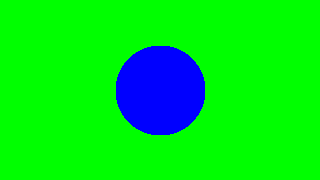
\includegraphics[scale=0.5]{spot}
\hfill

\includegraphics[scale=0.5]{spot04}

We have zoomed in $2\times$ (the spot is twice as big)
and our viewpoint is now above and to the right
of the spot.

You may want to add this to your function:
\begin{lstlisting}
def screenToWorld(i, j, width, height, center, radius):
    ....
    return (x, y)
\end{lstlisting}
Starting with \lstinline{spot03.py}, write 
\lstinline{spot04.py} that will allow us to
\begin{itemize}
\item resize the screen
\item recenter and zoom in (left button)
\item recenter and zoom out (right button)
\item recenter the view (any button but left and right)
\end{itemize}

Do this before going on!  \lstinline{spot04.py}
will be the basis for our Mandelbrot explorer,
which will be {\bf much} more interesting than
a blue spot!



\item[Making the pictures:]
The Mandelbrot set
pictures are made iterating the  Mandelbrot
function, described in the Wikipedia article.  
If the absolute value goes above 2,
then the series will diverge.  The algorithm simply counts
the number of steps until it goes above 2,
and colorizes according to the number of steps.  
If we go for 1000
iterations and it doesn't go above 2, we color it
black.

There is a pseudocode implementation of the
algorithm in the Wikipedia article.  Implement
this in Python with a function
\begin{lstlisting}
def mandelbrot(x0, y0):
\end{lstlisting}
that returns the number of iterations.

\lstinline{max_iterations} will be a global
variable.  We'll need it elsewhere.  (A value of
1000 is reasonable, but you can try other values.)

The colors I used in my Figures I got from 
\href{https://stackoverflow.com/questions/16500656/which-color-gradient-is-used-to-color-mandelbrot-in-wikipedia}{here}.
They are:
\begin{lstlisting}
    colors = [(66,  30,  15),
              (25,   7,  26),
              (9,   1,  47),
              (4,   4,  73),
              (0,   7, 100),
              (12,  44, 138),
              (24,  82, 177),
              (57, 125, 209),
              (134, 181, 229),
              (211, 236, 248),
              (241, 233, 191),
              (248, 201,  95),
              (255, 170,   0),
              (204, 128,   0),
              (153,  87,   0),
              (106,  52,   3)]
\end{lstlisting}
If the number of iterations is \lstinline{n},
we simply take \lstinline{colors[n % len(colors)]}
Unless, of course, \lstinline{n == max_iterations},
in which case we color it black.

\item[Making an image in pygame:]
I have provided a starter program in python
using the pygame library, called 
\lstinline{pygamecolors.py}, and provided
it in the lab folder.  Use this program
as your starting point for 
a program you will write called \lstinline{mandelbrot.py}.

\item[Changing colors to Mandelbrot colors:]
The provided program simply colorizes with a gradient
between the corners. You will have to compute
colors based on the Mandelbrot algorithm.

\item[Changing coordinates from screen to world:]
In coloring a pixel centered on \lstinline{(x,y)},
x and y are in {\bf screen coordinates}.  We
want x and y in terms of {\bf world coordinates}.
In this case, the world is the Mandelbrot
world of points in the plane.  To enable
this transformation, we will have two more
global variables: \lstinline{center}, which
will be a pair of real numbers giving the center
of the Mandelbrot scene, and \lstinline{radius}
which will be half the distance from 
the bottom to the top of the Mandelbrot scene.  Thus,
for example, if 
\begin{lstlisting}
center = (0.5, 0.5)
radius = 0.25
\end{lstlisting}
then the pixel in the center of the top row
will be at point 
\begin{lstlisting}
(0.5, 0.5 + radius) = (0.5, 0.75)
\end{lstlisting}
and the pixel in the center of the bottom
row will be at point 
\begin{lstlisting}
(0.5, 0.5 = radius) = (0.5, 0.25)
\end{lstlisting}

The pixel at the center of the left edge will
depend on the aspect ratio of the image.
If the image is, for example, 640 wide
and 480 tall, then the aspect ratio is
$640/480 \approx 1.33$.  The pixel at the
center of the left edge, therefore, will be
at 
\begin{lstlisting}
(0.5 - aspectRatio*radius, 0.5) =  (1.666, 0.5)
\end{lstlisting}
Write a function in python
that will transform screen coordinates to 
world (Mandelbrot space) coordinates.
It will look like this:
\begin{lstlisting}
def screenToWorld(i, j, screen, center, radius):
    w,h = screen.get_size()
    ...
    return (x,y)
\end{lstlisting}
Where \lstinline{(x,y)} are the corresponding
points in world space.

As a test, with center and radius as above,
and aspect ratio of 640/480, I got the following
numbers for these values of i and j:
\begin{lstlisting}
(0,0)=> (0.16666666666666669, 0.75)
(0,50)=> (0.16666666666666669, 0.6979166666666666)
(0,100)=> (0.16666666666666669, 0.6458333333333333)
(50,0)=> (0.21875, 0.75)
(50,50)=> (0.21875, 0.6979166666666666)
(50,100)=> (0.21875, 0.6458333333333333)
(100,0)=> (0.27083333333333337, 0.75)
(100,50)=> (0.27083333333333337, 0.6979166666666666)
(100,100)=> (0.27083333333333337, 0.6458333333333333)
\end{lstlisting}

\item[Mouse navigation:] If you start with a center
of (0,0) and a radius of 2 you should see
the entire set (remember that any point farther
than 2 from the origin cannot be in the set).

How can we look at other regions?  We will use the mouse.
The position of the mouse click will determine the new center
(translated from screen to world coordinates, of course!)

We will zoom in with the left mouse button and zoom
out with the right mouse button.  Zooming in just means
the radius is divided by 2.  Zooming out just
means the radius is multiplied by two.

The file I've provided, called \lstinline{testmouse.py}
shows you how to check on mouse events. 
Run it and then click in the window, using
any of your mouse buttons, watching
what is printed on the console.  This should happen
the same place you check for keyboard events!  Which
should happen once and only once per loop!  The keyboard
and mouse events are all stored in a single queue.

The middle button, if you have one, should recenter
the scene but not zoom in or out.  If you don't have
a middle button, don't worry.  It will probably work, 
anyway!

\item[Black is slow!]  The black areas inside
the Mandelbrot set are the ones where the algorithm
had to go to the maximum number of iterations.
These are clearly going to be the slowest points.
If you select regions without so much black,
they'll render faster.

\end{description}
\newpage

\centerline{\Large \bf Gallery}

\showfig{mandX-0.688Y0.382R0.00390625.png}

\showfig{mandX-0.694Y-0.356R0.0078125.png}

\showfig{mandX-0.670Y-0.458R0.0078125.png}


\showfig{mandX-0.707Y-0.353R0.015625.png}


\showfig{mandX-1.624Y0.002R0.125.png}


\showfig{mandX0.456Y0.111R0.0625.png}


\showfig{mandX0.464Y-0.360R0.0625.png}


\end{document}
